\documentclass[12pt]{exam}
\usepackage[icp]{template-for-exam}
\usepackage{textpos}
\usepackage{pgfplots}
\pgfplotsset{
  compat=1.18, 
  every axis/.append style={
    ylabel = {distance (meters)},
    xlabel={time (seconds)},
    grid=both,
    major grid style = ultra thick,
    minor grid style = thin,
  },
}

\title{Car Lab Warmup}
\author{Rohrbach}
\date{\today}

\begin{document}
\maketitle

\begin{questions}

  \question 
    Calculate the average for each of these data sets:

    \begin{parts}
      \part 
        \begin{tabular}{|ccc|}
          \hline
          1.35 & 1.58 & 1.24 \\
          \hline
        \end{tabular}
        \vs

        \part 
        \begin{tabular}{|ccc|}
          \hline
          10.12 & 9.98 & 9.85 \\
          \hline
        \end{tabular}
        \vs


    \end{parts}

  \question Draw a best-fit line for this graph.  


  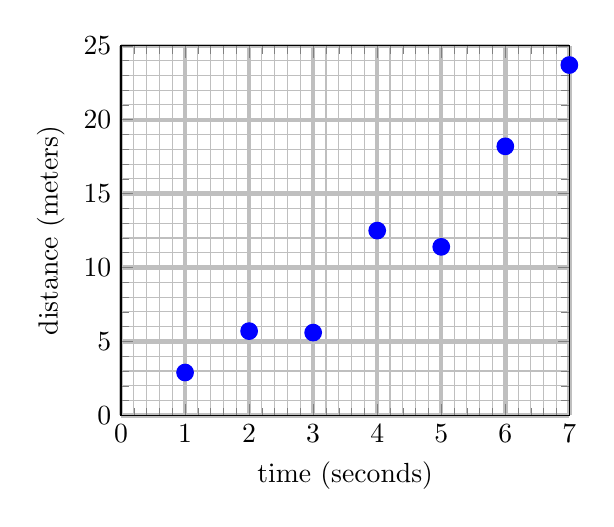
\begin{tikzpicture}
    \begin{axis}[
        xmin=0, xmax=7,
        ymin=0, ymax=25,
        xtick={0,...,10},
        ytick={0,5,10,15,20,25,30},
        grid=both,
        minor x tick num = 4,
        minor y tick num = 4,
        width=.6\textwidth
    ]
    
      \addplot [only marks, blue, mark size=3pt] table {
        x   y
        1   2.9
        2   5.7
        3   5.6
        4   12.5
        5   11.4
        6   18.2
        7   23.7
        8   21.5
        9   28.1
        10  21.8
      };
      
    \end{axis}
  \end{tikzpicture}

  \pagebreak
  \question 
    Plot these points on a graph and then draw a best 
    fit line.

    \begin{center}
          \begin{tabular}{|c|c|}
            \hline
            \bf time &  \bf dist \\
              (s)    &     (m)   \\
            \hline\hline
              0.6    &   0.5  \\\hline
              3.1    &   1.0  \\\hline
              5.8    &   1.5  \\\hline
              7.9    &   2.0  \\\hline
              9.4    &   2.5  \\\hline
              12.2   &   3.0  \\\hline
          \end{tabular}
    \end{center}

    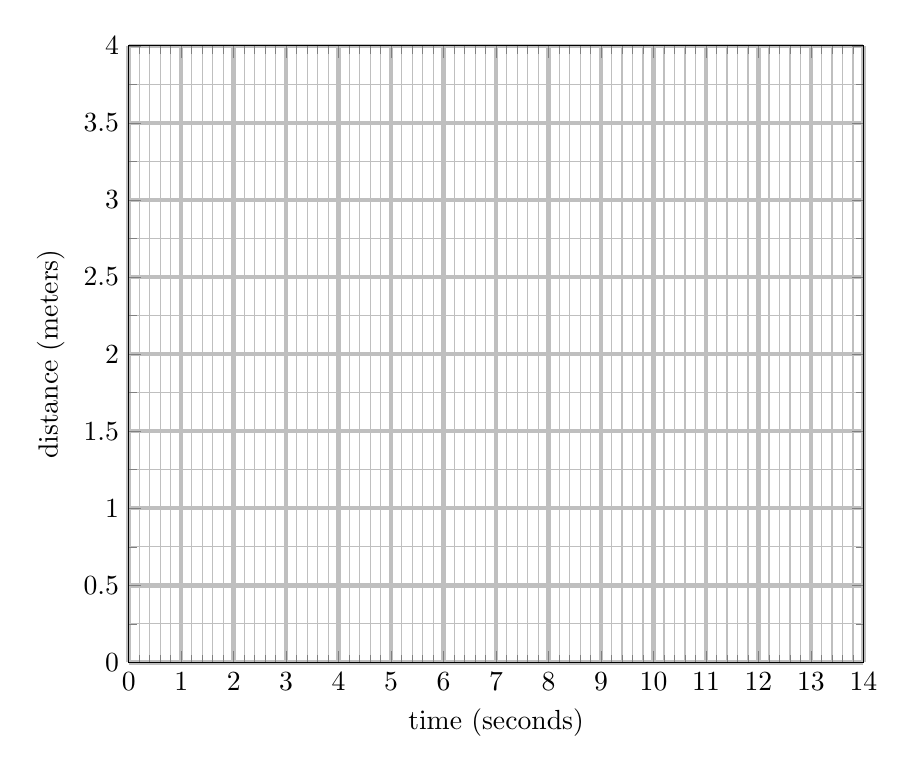
\begin{tikzpicture}
      \begin{axis}[
          xmin=0, xmax=14,
          ymin=0, ymax=4,
          xtick={0,...,15},
          minor x tick num = 4,
          ytick={0,0.5,1,1.5,2,2.5,3,3.5,4,4.5},
          minor y tick num = 1,
          width=.9\textwidth,
      ]
      
        % \addplot [only marks, mark=*, mark size=2pt, color=blue] table {
        %     x    y
        %     0.6  0.5
        %     3.1  1.0
        %     5.8  1.5
        %     7.9  2.0
        %     9.4  2.5
        %     12.2 3.0
        % };
      \end{axis}
    \end{tikzpicture}
  
    

    
    


\end{questions}
\end{document}